\documentclass{beamer}

\usepackage{listings}
\usepackage{xcolor}
\usepackage{multicol}
\usepackage{amsmath}
\usepackage{subcaption}

\definecolor{codegreen}{rgb}{0,0.6,0}
\definecolor{codegray}{rgb}{0.5,0.5,0.5}
\definecolor{codepurple}{rgb}{0.58,0,0.82}
\definecolor{backcolour}{rgb}{0.95,0.95,0.92}

\lstdefinestyle{mystyle}{
    %backgroundcolor=\color{backcolour}, 
    commentstyle=\color{codegreen},
    keywordstyle=\color{magenta},
    numberstyle=\tiny\color{codegray},
    stringstyle=\color{codepurple},
    basicstyle=\ttfamily\footnotesize,
    breakatwhitespace=false,         
    breaklines=true,                 
    captionpos=b,                    
    keepspaces=true,                 
    numbers=left,                    
    numbersep=5pt,                  
    showspaces=false,                
    showstringspaces=false,
    showtabs=false,                  
    tabsize=2
}

\lstset{style=mystyle}

\usepackage{hyperref}
\hypersetup{
    colorlinks=true,
    linkcolor=blue,
    filecolor=magenta,      
    urlcolor=cyan
}

\urlstyle{same}

\title{3: Complete Search, Divide and Conquer, Greedy}
\author{CPCFI}
\institute{UNAM's School of Engineering}
\date{2021 \\ \vspace{0.5cm} \scriptsize{Based on: Halim S., Halim F.\textit{Competitive Programming 3}}. Handbook for ACM ICPC and IOI Contestants. 2013}

\begin{document}

\frame{\titlepage}

\AtBeginSection[]
{
  \begin{frame}
    \frametitle{Table of Contents}
    \tableofcontents[currentsection]
  \end{frame}
}

%-------------------------------------------------------------------------------------------
%-------------------------------------------------------------------------------------------
%-------------------------------------------------------------------------------------------
\section{Introduction to algorithmic heuristics}
\begin{frame}[fragile]
\frametitle{Background}

In general, we have two types of algorithmic problems:
\begin{enumerate}
    \item \textbf{Optimization}: we'd like to find a minimum or maximum within a \textit{search space}
    \item \textbf{Decision}: we'd like to answer 'yes' or 'no' for a problem within a \textit{search space}
\end{enumerate}

\end{frame}


\begin{frame}[fragile]
\frametitle{Algorithmic examples}

For example:
\begin{itemize}
    \item \textbf{Sudoku}: given a sudoku board with some numbers, decide whether or not a solution exists
    \item \textbf{Bipartite graph}: given a graph $G$, decide if a partition of its vertices exists such that $G$ is bipartite
    \item \textbf{Robotic arm}: given some points in a plane, we'd like to find a Hamiltonian cycle of minimum length that goes through all points
\end{itemize}

\end{frame}

\begin{frame}[fragile]
\frametitle{Search Space}

\textbf{Definition}: the state's space for a problem (optimization or decision) is the set of all possible configurations or inputs we must consider in order to answer the problem.

\vspace{0.5cm}

\begin{itemize}
    \item Numbers from $1$ to $n$
    \item Permutations of $n$ elements
    \item Sets of $n$ elements
    \item For a given $k$, all subsets of size $k$ from $n$ possible elements
    \item Vectors of $m$ elements taken from a set of $n$ elements
\end{itemize}

\end{frame}

\begin{frame}[fragile]
\frametitle{Example \#0}

\vspace{0.3cm}
Given a list of $n$ integers, we'd like the following:
\begin{itemize}
    \item Decide if two numbers exist such that its sum equals $1000$
    \item Decide which two numbers have the minimum sum
\end{itemize}

\vspace{0.5cm}
*The first problem is a \color{blue}decision \color{black} problem, while the second is an \color{blue}optimization \color{black} problem.

\end{frame}


\begin{frame}[fragile]
\frametitle{Algorithmic heuristics}

Once we know the type of algorithmic problem (optimization or decision) and the search space $S$, we can start looking for the optimal solution (or correct solution) within $S$. For this, we can use the following heuristics:

\vspace{0.3cm}

\begin{itemize}
    \item Explore the search space $S$
    	\begin{itemize}
		    \item \color{blue}Complete Search (Brute Force)\color{black}: explore all the elements of $S$
		    \item Pruning: explore only the elements of $S$ that we know have a possibility of being the optimal or correct solution 
		\end{itemize}
    \item Divide and Conquer
    \item Greedy algorithms
    \item Dynamic Programming \footnote{We look into this heuristic in slides \#4 and \#5}
\end{itemize}

\end{frame}


%-------------------------------------------------------------------------------------------
%-------------------------------------------------------------------------------------------
%-------------------------------------------------------------------------------------------
\section{3.2 Complete Search}

\begin{frame}[fragile]
\frametitle{3.2 Complete Search}
The idea: 

\begin{figure}
    \centering
    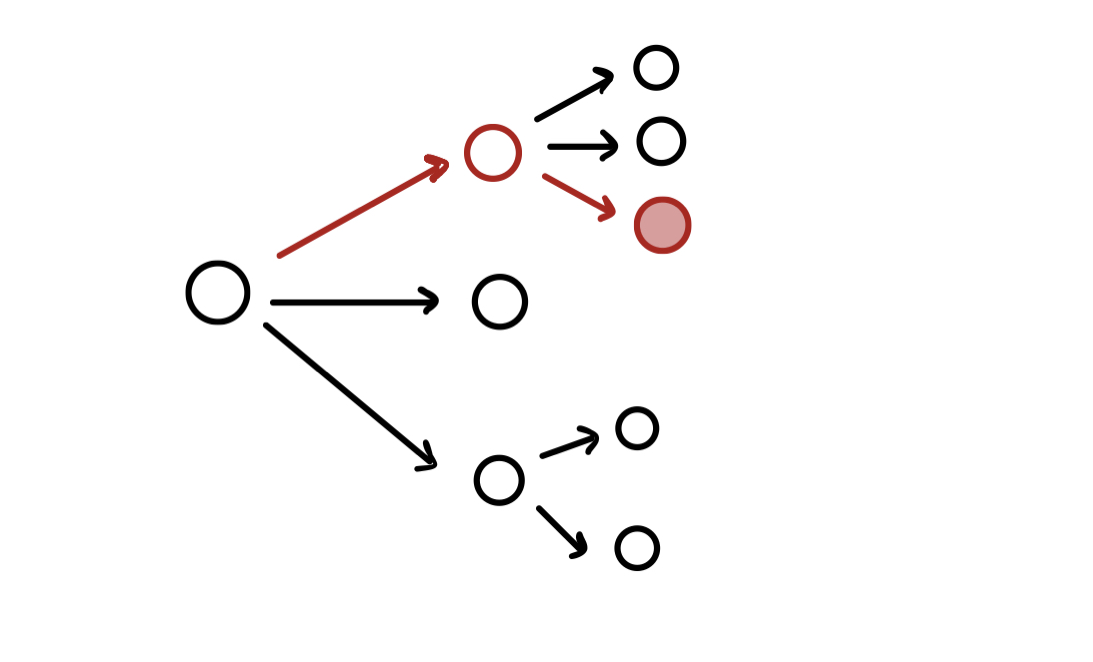
\includegraphics[scale=0.2]{imgs/complete_search.png}
\end{figure}

\end{frame}


\begin{frame}[fragile]
\frametitle{Complete Search}

\begin{itemize}
    \item Heuristic for solving a problem by traversing through the entire (or part of) the search space to obtain a correct solution
    \item Also known as \textit{brute force} or \textit{recursive backtracking}
    \item During the search, one could prune the search space (\color{blue}Pruning technique\color{black}) by only traversing through possible solutions and ignoring solutions that have no possibility of containing the correct solution
\end{itemize}

\end{frame}

\begin{frame}[fragile]
\frametitle{Complete Search}

One should develop a complete search solution when:
\begin{enumerate}
    \item No other clear algorithm exists
    \item A better algorithm exists but are too complex for a small input size \footnote{For example, Range Minimum Queries on static arrays with $N < 100$ is solvable with $O(N)$ loop for each query} 
\end{enumerate}

\vspace{1cm}

\color{blue} In ICPC, Complete Search should be the first solution considered as it is usually a simple technique to code and debug.\color{black}

\end{frame}

\begin{frame}[fragile]
\frametitle{Complete Search on ICPC}
\begin{itemize}
    \item Complete Search should never get the Wrong Answer (WA) veredict since it always finds the correct solution. However, time limit exceeded (TLE) is very common to occur since it's a slow technique
    \item One should do a proper analysis before implementing Complete Search
\end{itemize}
Recall the following table: 
\begin{figure}
    \centering
    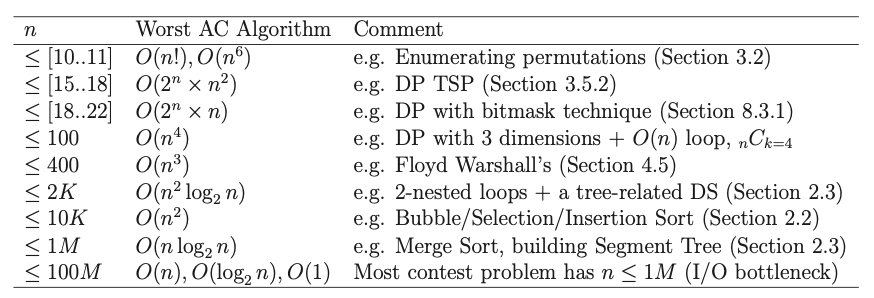
\includegraphics[scale=0.3]{imgs/complexities_table.png}
\end{figure}
\end{frame}

\begin{frame}[fragile]
\frametitle{3.2.1 Iterative Complete Search - Example \#1}

\begin{itemize}
	\item \href{https://onlinejudge.org/index.php?option=com_onlinejudge&Itemid=8&category=9&page=show_problem&problem=666}{UVa 725 - Division}
    \item C++ code: \color{red}\verb|/CompleteSearch/275.cpp|\color{black}
\end{itemize}

\vspace{0.5cm}

\color{red}\textbf{Problem description}\color{black}\\ 

Write a program that finds and displays all pairs of $5$-digit numbers that between them use the digits $0$ through $9$ once each, such that the first number divided by the second is equal to an integer $N$, where $2 \leq N \leq 79$. That is, $$\frac{abcde}{fghij} = N$$ where each letter represents a different digit. The first digit of one of the numerals is allowed to be zero.

\end{frame}

\begin{frame}[fragile]
\frametitle{Iterative Complete Search - Example \#2}

\begin{itemize}
	\item \href{https://onlinejudge.org/index.php?option=com_onlinejudge&Itemid=8&category=6&page=show_problem&problem=382}{UVa 441 - Lotto}
    \item C++ code: \color{red}\verb|/CompleteSearch/441.cpp|\color{black}
\end{itemize}

\vspace{0.5cm}

\color{red}\textbf{Problem description}\color{black}\\ 
Given $6 < k < 13$ integers, enumerate all possible subsets of size $6$ of these integers in sorted order. Since the size of the required subset is always $6$ and the output has to be sorted lexico-graphically (the input is already sorted), the easiest solution is to use six nested loops. Even when $k = 12$, we only have: $$C_6(12) = \begin{pmatrix} 12 \\ 6\end{pmatrix} = \frac{12!}{6!\cdot(12-6)!} = 924$$ combinations

\end{frame}

\begin{frame}[fragile]
\frametitle{Iterative Complete Search - Example \#3}

\begin{itemize}
    \item \href{https://onlinejudge.org/index.php?option=com_onlinejudge&Itemid=8&category=27&page=show_problem&problem=2612}{UVa 11565 - Simple Equations}
    \item C++ code: \color{red}/CompleteSearch/11565.cpp\color{black}
\end{itemize}

\vspace{0.5cm}

\color{red}\textbf{Problem Description}\color{black}\\

Given three integers $A,B,C$ ($1 \leq A,B,C \leq 10000$), find three other \textbf{distinct} integers $x,y,z$ such that $x+y+z=A$, $x\times y\times z=B$ and $x^2 + y^2 + z^2=C$.

\vspace{0.5cm}

\textbf{Hint:} We must avoid three nested loops from $1 \rightarrow 10000$?

\end{frame}

\begin{frame}[fragile]
\frametitle{3.2.2 Recursive Complete Search}

Before we look into these examples, we must study \color{blue}\textbf{Backtracking}\color{black}

\end{frame}

%-------------------------------------------------------------------------------------------
%-------------------------------------------------------------------------------------------
%-------------------------------------------------------------------------------------------
\subsection{Backtracking}
\begin{frame}[fragile]
\frametitle{Backtracking - Definition}

\textbf{Definition:} backtracking is a systematic way of running through all possible configurations of a search space. 

\vspace{0.3cm}

\begin{itemize}
    \item Regarding the type of search space, all search spaces must generate each possible configuration \textbf{exactly once}
    \item In order to avoid repetitions and missed configurations, we must define a systematic generation order
\end{itemize} 
\end{frame}

\begin{frame}[fragile]
\frametitle{Backtracking - The Idea}

\begin{itemize}
    \item Backtracking models the combinatorial solution by using a vector $a = (a_1, a_2, \ldots, a_n)$ where each element $a_i$ is selected from a finite ordered set $S_i$
    \item The vector $a$ represents the solution
    \item At each step in the backtracking algorithm, we try to extend $a$ by adding another element at the end
    \item \color{blue}Backtracking constructs a tree of partial solutions\color{black}
\end{itemize}

\end{frame}

\begin{frame}[fragile]
\frametitle{Backtracking - Algorithm}

\begin{lstlisting}
Backtrack(a,k)
if a=(a1,a2,...,an) is a solution
	Report it
else
	k=k+1
	construct Sk //set of candidates for position k of a
	while Sk has elements
		ak = an element in Sk
		Sk = Sk - {ak}
		Backtrack(a,k)
\end{lstlisting}

\end{frame}

\begin{frame}[fragile]
\frametitle{Backtracking - Examples: Subsets}

\textbf{Problem}: Find the subsets of an $n$-element set. For example, the integers $\{1,\ldots, n\}$ \\ \vspace{0.4cm}

For $n=1$: \\ \hspace{0.5cm} $2^1$ subsets: $\{\}, \{1\}$ \\
For $n=2$: \\ \hspace{0.5cm} $2^2$ subsets: $\{\}, \{1\}, \{2\}, \{1,2\}$ \\
For $n=3$: \\ \hspace{0.5cm} $2^3$ subsets: $\{\}, \{1\}, \{2\}, \{3\}, \{1,2\}, \{1,3\}, \{2,3\}, \{1,2,3\}$ \\

$\vdots$ \\ \vspace{0.2cm}
For $n=k$: \\ \hspace{0.5cm} $2^k$ subsets \\ \vspace{0.3cm}

C++ code: \color{red}\verb|/CompleteSearch/backtracking_subsets.cpp|\color{black}

\end{frame}


\begin{frame}[fragile]
\frametitle{Backtracking - Examples: Permutations}

\textbf{Problem}: Generate all permutations of $n$ integers: $\{1,\ldots,n\}$ \\ \vspace{0.2cm}

For $n=1$: $\{0\}$ \\

For $n=2$: $\{01, 10\}$ \\

For $n=3$: $\{012, 021, 102, 120, 201, 210\}$ \\ 

$\vdots$ \\


C++ code: \color{red}\verb|/CompleteSearch/backtracking_permutations.cpp|\color{black}

\end{frame}


%-------------------------------------------------------------------------------------------
\begin{frame}[fragile]
\frametitle{Recursive Complete Search - Example \#4}
	\begin{itemize}
	    \item \href{https://onlinejudge.org/index.php?option=com_onlinejudge&Itemid=8&category=9&page=show_problem&problem=691}{UVa 750 - 8 Queens Chess Problem}
	    \item C++ code: \color{red}\verb|/CompleteSearch/750.cpp|\color{black}
	\end{itemize}
	\vspace{0.4cm}
	\color{red}\textbf{Problem Description}\color{black} \\
	In chess (with an $8 \times 8$ board), it is possible to place eight queens on the board such that no two queens attack each other. Determine all such possible arrangements given the position of one of the queens (i.e. coordinate $(a, b)$ must contain a queen).
	
	\begin{figure}
	    \centering
	    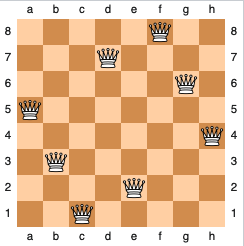
\includegraphics[scale=0.35]{imgs/8queen.png}
	\end{figure}
\end{frame}


\begin{frame}[fragile]
\frametitle{Recursive Complete Search - Example \#5}

\begin{itemize}
	\item UVa 11195 - Another n-Queen Problem
    \item \color{red}\verb|C++ code: /CompleteSearch/11195.cpp|\color{black}
\end{itemize}

\color{red}\textbf{Problem Description}\color{black} \\
Given an $n \times n$ chessboard ($3 < n < 15$) where some of the cells are bad (queens cannot be placed on those bad cells), how many ways can you place n queens in the chessboard so that no two queens attack each other? Note: Bad cells cannot be used to block queens’ attack.

\end{frame}

\begin{frame}[fragile]
\frametitle{Recursive Complete Search - Example \#5}

\begin{itemize}
    \item The recursive backtracking algorithm presented for the 8-Queen problem is not fast enough for $n=14$
    \item It's too slow when checking whether the position of a new queen is valid since we compare the new queen's position with the previous $c-1$ queens' positions
    \item Therefore, we must store the same information with three boolean arrays
    	\begin{itemize}
		    \item \verb|rw|: represents the $n$ rows
		    \item \verb|ld|: $2\times n-1$ left diagonals
		    \item \verb|rd|: $2\times n-1$ right diagonals
		\end{itemize}
\end{itemize}

\end{frame}

\begin{frame}[fragile]
\frametitle{Recursive Complete Search - Example \#5}

\begin{itemize}
    \item When a queen is placed at $(r,c)$ we flag \color{blue}\verb|rw[c] = true| \color{black} to prevent this \textbf{row} from being used again
    \item In addition to this, we need to prevent its left and right \textbf{diagonals} from being used:
    	\begin{itemize}
		    \item If another queen $(a,b)$ is placed in either a right or left diagonal of the original queen $(r,c)$, then the following equation is satisfied: $$\text{abs}(r-a) = \text{abs}(c-b)$$ $$r-c = a-b \quad\quad\text{or}\quad\quad r+c=a+b$$
		    \item Since $r-c$ can be negative, we must add an offset of $n+1$
		    \item Therefore, we flag \color{blue}\verb|ld[r-c+n+1]=true| \color{black} and \color{blue}\verb|rd[r+c]=true| \color{black} if a queen is placed at $(r,c)$
		\end{itemize}
\end{itemize}

\end{frame}


\begin{frame}[fragile]
\frametitle{3.2.3 Tips}

\begin{itemize}
    \item One of the biggest problems with Complete Search is whether your solution will pass in the right amount of time or will get a Time Limit Exceeded (TLE) verdict
    \item Now, we'll review some tips to consider when designing a Complete Search solution
\end{itemize}

\end{frame}

\begin{frame}[fragile]
\frametitle{Tip \#1: Filtering vs. Generating}

\color{blue}\textbf{Filters}\color{black}: programs that examine most of the candidate solutions and choose the correct ones \\ \vspace{0.3cm}

\color{blue}\textbf{Generators}\color{black}: programs that gradually build the solutions and immediately prune invalid or partial solutions \\ \vspace{0.3cm}

\begin{itemize}
    \item Filters are easier to code but run slower since it's much harder to prune the search space iteratively
    \item Before programming a generator, do an algorithm analysis to know if a filter is good enough
\end{itemize}
	
\end{frame}

\begin{frame}[fragile]
\frametitle{Tip \#2: Prune Death Ends Early}

\begin{itemize}
    \item When generating solutions using recursive backtracking (recall UVa 750 - 8-queens problem) we might encounter partial solutions that we know will never produce a correct solution
    	\begin{itemize}
		    \item For example, suppose we have an initial queen at \verb|row[0]=2|. Knowing this, we know that any board configuration with queens at \verb|row[1] = 1| or \verb|row[1]=0| will never produce correct solutions, thus, we must stop at this point and focus on the next possible solutions (\verb|row[1] != {0,1,2}|)
		\end{itemize}
    \item We need to identify this paths as early as possible and stop the search at that point
    \item \color{blue}The earlier you prune the search space, the better\color{black}
\end{itemize}

\end{frame}

\begin{frame}[fragile]
\frametitle{Tip \#3: Exploit symmetries}

\begin{itemize}
    \item We must exploit problem domain symmetries to reduce execution time
	\item Using symmetries could increase code complexity and thus time debugging
	\item \color{blue}Exploit symmetries only if the reduced time is significant\color{black}
\end{itemize}

\end{frame}

\begin{frame}[fragile]
\frametitle{Tip \#4: Optimize Your Source Code I}

\begin{enumerate}
    \item If possible, use C++ instead of Java since it's faster
    \item Use \verb|scanf/printf| instead \verb|cin/cout|
    \item Use C++ STL \verb|algorithm::sort|
    \item Access a 2D array row by row; it's faster
    \item Bit manipulation on the built-in integer data types is more efficient that index manipulation in a boolean array
    \item Use lower level data structures (or types) at all times if you do not need the extra functionality of the higher level ones. For example, use an \verb|array| with a slightly larger size than the maximum input size instead of a resizable array (\verb|vector|)    
\end{enumerate}

\end{frame}

\begin{frame}[fragile]
\frametitle{Tip \#4: Optimize Your Source Code II}

\begin{enumerate}
	\setcounter{enumi}{6}
	\item Declare most data structures once by placing them in a global scope and allocate enough memory to deal with the largest input of the problem. This way we do not need to pass data structures around as function arguments
    \item If possible, write your code iteratively instead of recursively
    \item If you have an array \verb|A| and you frequently access the value \verb|A[i]| within nested loops, then, a better option would be to declare a variable \verb|temp = A[i]| and work with \verb|temp| instead
    \item Appropriate usage of macros or inline functions can reduce time
    \item Using C-style character arrays will perform better than using the C++ STL \verb|string| class
    
\end{enumerate}

\end{frame}

\begin{frame}[fragile]
\frametitle{Tip \#5: Iterative vs. Recursive Complete Search I}

If a problem is solvable by Complete Search, it will also be clear when to use the iterative or recursive backtracking approaches:

\begin{enumerate}
    \item \textbf{Iterative} approaches are used when it's easy to derive the different states or all states have to be checked
    	\begin{itemize}
		    \item \textit{Subsets, permutations, etc}
		\end{itemize}
	\item \textbf{Recursive} approaches are used when it's hard to derive states with a simple index or when one wants to prune the search space
    	\begin{itemize}
		    \item \textit{$n$-queens problem, etc}
		\end{itemize}
\end{enumerate}

\end{frame}

\begin{frame}[fragile]
\frametitle{Tip \#5: Iterative vs. Recursive Complete Search II}

\color{blue}If the search space of a problem - that can be solved using Complete Search - is large, then recursive backtracking approaches that allow early pruning of infeasible sections are usually better\color{black}

\end{frame}


%-------------------------------------------------------------------------------------------
%-------------------------------------------------------------------------------------------
%-------------------------------------------------------------------------------------------
\subsection{UVa - 3.2}
\begin{frame}[fragile]
\frametitle{UVa - Online Judge}
	\begin{itemize}
	    \item Complete Search Problems: \url{https://onlinejudge.org/index.php?option=com_onlinejudge&Itemid=8&category=639}
	    \item If \textbf{UVa Online Judge} is not working, please refer to \cite{Halim}: page 80
	\end{itemize}
\end{frame}


%-------------------------------------------------------------------------------------------
%-------------------------------------------------------------------------------------------
%-------------------------------------------------------------------------------------------
\section{3.3 Divide and Conquer}

\begin{frame}[fragile]
\frametitle{3.3 Divide and Conquer - The Idea}

\begin{figure}
    \centering
    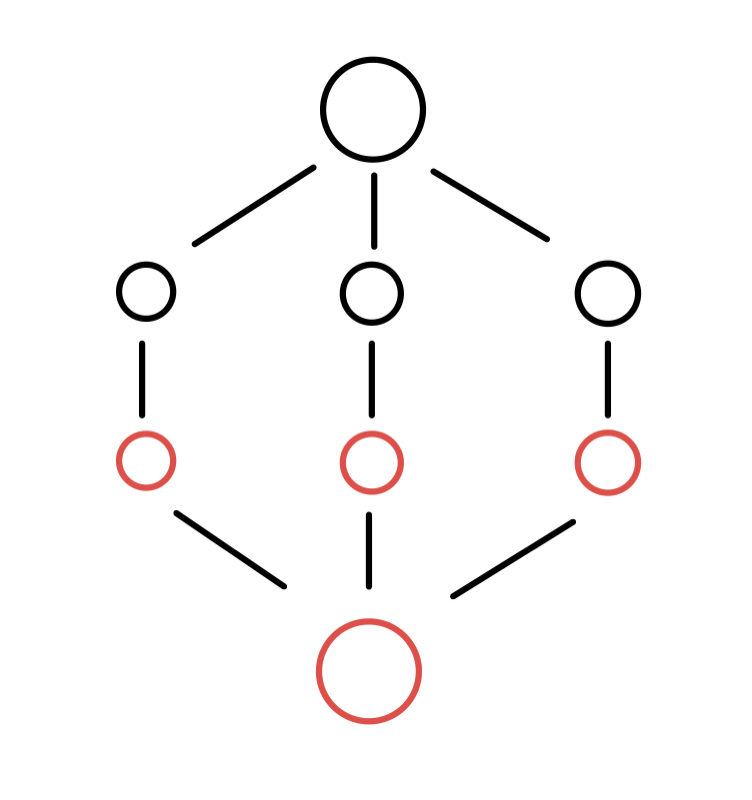
\includegraphics[scale=0.25]{imgs/divide_and_conquer.jpeg}
\end{figure}

\end{frame}

\begin{frame}[fragile]
\frametitle{Divide and Conquer - Definition}

Divide and Conquer (DQ) is a problem solving paradigm in which a problem is divided into smaller parts and then each part is solved (conquered). The general steps are the following:
\vspace{0.3cm}
\begin{enumerate}
    \item \textbf{Divide} the original problem into sub-problems - usually in halves
    \item \textbf{Solve} each of these sub-problems - which are now easier
    \item \textbf{Combine} these solutions to obtain a complete solution of the problem
\end{enumerate}

\end{frame}

\begin{frame}
\frametitle{Divide and Conquer - Examples}

Some examples of DQ:

\begin{itemize}
    \item Quick Sort
    \item Merge Sort
    \item Heap Sort
    \item Binary Search
\end{itemize}

\end{frame}

\begin{frame}[fragile]
\frametitle{3.3.1 Interesting Usages of Binary Search}

Binary Search algorithm is an example of the Divide and Conquer paradigm; however, there are other ways in which this algorithm could be used: 

\begin{itemize}
    \item Ordinary Usage
    \item On Uncommon Data Structures
    \item Bisection Method
    \item Binary Search the Answer
\end{itemize}

\end{frame}

\begin{frame}[fragile]
\frametitle{Binary Search - Ordinary Usage}

\begin{itemize}
    \item The canonical way of using \textit{Binary Search} is searching for an item in a \textit{static sorted array}
    \item We check the middle element of the sorted array to determine if it contains the element we are searching
    \item If not, we can decide whether the answer is to the left or the right of the middle element
    \item On each iteration, we are halving the space search, thus the complexity is $O(\log n)$
\end{itemize}

\end{frame}

\begin{frame}[fragile]
\frametitle{Binary Search On Uncommon Data Structures - Problem}

\textbf{Problem description}\footnote{'My Ancestor' was used in the Thailand ICPC National Contest 2009}: Given a weighted tree of up to $N$ vertices ($N \leq 80K$) where vertex values increase from root to leaves on each level of the tree, find the ancestor vertex closest to the root from a starting vertex $v$ that has weight at least $P$. Find these ancestors for $Q$ queries ($Q \leq 20K$); each query contains a vertex $v$.

\begin{figure}
    \centering
    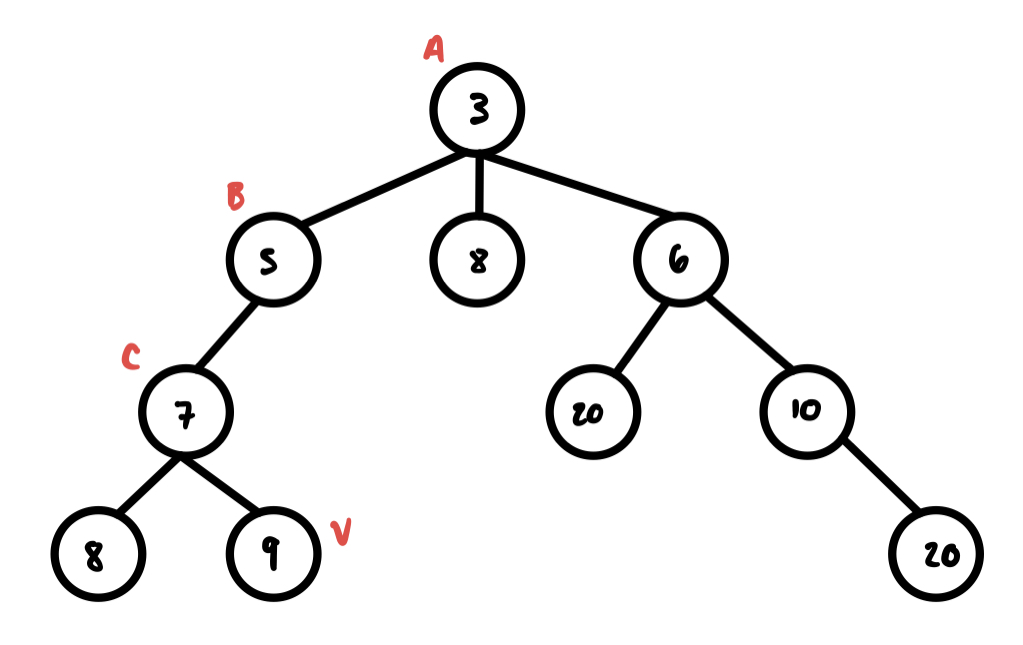
\includegraphics[scale=0.15]{imgs/my_ancestor.jpeg}
    \caption{My Ancestor problem}
\end{figure}

\end{frame}

\begin{frame}[fragile]
\frametitle{Binary Search On Uncommon Data Structures - Naive Solution}

\textbf{Naive Solution}: perform linear scan per query in $O(N)$. Starting from a vertex $v$ we move up in the tree until we reach the first vertex $u$ whose direct parent has value $< P$ or until we reach the root. If vertex $u$ has value $\geq P$ and $u \neq v$, we have found the solution. \\ \vspace{0.3cm}

Since there are $Q$ queries, we have $O(QN)$ complexity which will get a TLE verdict since $80,000\cdot20,000 = 1,600,000,000$ \\ \vspace{0.3cm}

\color{blue}*Recall that modern computers can run up to $100M$ operations per second.\color{black}

\end{frame}

\begin{frame}[fragile]
\frametitle{Binary Search On Uncommon Data Structures - Better Solution}

\textbf{Better solution}: 

\begin{enumerate}
    \item Store the $Q$ queries\footnote{The important element to store is the $v$ vertex from which we're going to start}
    \item Traverse the tree just once using preorder tree traversal and store the partial \textit{root-to-current-vertex sequence}
    \item When we land on a queried vertex $v$, we can perform a binary search in $O(\log N)$ to obtain the ancestor closest to the root with a value of at least $P$ and store the solution
    \item Perform a $O(Q)$ iteration to output the results; the overall complexity of this solution is $O(Q\log N)$ \\ \vspace{0.3cm}
    \color{blue}$Q\log N = 20,000 \log(80,0000) \approx 98,000$ \\ $98,000 << 1,600,000,000$\color{black}
\end{enumerate}

\end{frame}

\begin{frame}[fragile]
\frametitle{Binary Search On the Bisection Method}

\begin{itemize}
    \item Binary Search principle can also be used to find the root of a function that may be difficult to compute directly
    \item The bisection method takes $O(\log_2(\frac{b-a}{\epsilon})))$ to get an answer that is good enough
\end{itemize}

\end{frame}

\begin{frame}[fragile]
\frametitle{Binary Search the Answer - Problem}

\textbf{Problem description\footnote{UVa 11935}}: Imagine that you are an explorer trying to cross a desert. You use a jeep with a large enough fuel tank – initially full. You encounter a series of events throughout your journey such as \textit{drive}, \textit{gas leak}, \textit{encounter gas station}, \textit{encounter a mechanic} or \textit{reach your destination}. You need to determine the smallest possible fuel tank capacity for your jeep to be able to reach the goal. The answer must be precise to three digits after decimal point.

\end{frame}

\begin{frame}[fragile]
\frametitle{Binary Search the Answer - Solution}

\begin{itemize}
    \item From the problem description, the range of possible answers is between $[0, \ldots, 10000]$, with 3 digits of precision. However, there are $10M$ such possibilities. Trying each value sequentially will get us a TLE verdict
    \item However, this problem has a property we can exploit. Suppose the correct answer is $X$:
    	\begin{itemize}
		    \item Setting the jeep's fuel capacity to any value between $[0,\ldots,X-0.001]$ will not bring the jeep to the goal event
		    \item Setting the jeeps' fuel capacity to any value between $[X,\ldots,10000]$ will bring the jeep to the goal event
		\end{itemize}
	\item C++ code: \color{red}\verb|/DivideAndConquer/11935.cpp|\color{black}
\end{itemize}

\end{frame}

\begin{frame}
\frametitle{Divide and Conquer - In Programming Contests}

\begin{itemize}
    \item The most common use case of the Divide and Conquer paradigm, is the Binary Search Principle
\end{itemize}

\end{frame}

%-------------------------------------------------------------------------------------------
%-------------------------------------------------------------------------------------------
%-------------------------------------------------------------------------------------------
\subsection{UVa - 3.3}
\begin{frame}[fragile]
\frametitle{UVa - Online Judge}
	\begin{itemize}
	    \item Divide and Conquer problems: \url{https://onlinejudge.org/index.php?option=com_onlinejudge&Itemid=8&category=660}
	    \item If this link is not working, please check \cite{Halim}: page 88 for DQ Problems
	\end{itemize}
\end{frame}


%-------------------------------------------------------------------------------------------
%-------------------------------------------------------------------------------------------
%-------------------------------------------------------------------------------------------
\section{3.4 Greedy}
\begin{frame}[fragile]
\frametitle{3.4 Greedy - The Idea}

\begin{figure}
    \centering
    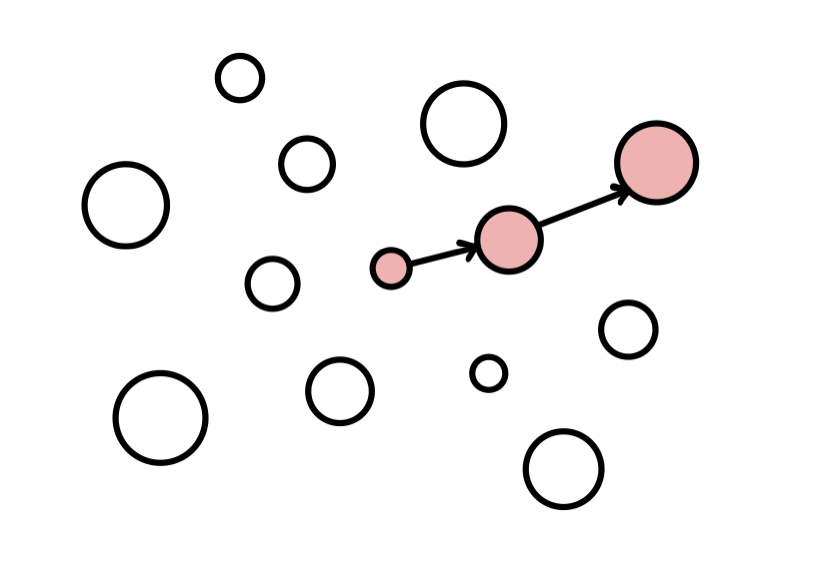
\includegraphics[scale=0.25]{imgs/greedy.jpeg}
    \caption{Choosing the best local option hoping to reach the best global solution}
\end{figure}

\end{frame}

\begin{frame}[fragile]
\frametitle{Greedy - Definition}

An algorithm is said to be \color{blue}greedy \color{black} if it makes the locally optimal choice at each step hoping to eventually reach the globally optimal solution. In some cases greedy works but in many others, it does not. \\

\vspace{0.3cm}

\color{blue}\textbf{Note:} finding a greedy solution is an art, just as finding good Complete Search solutions requires creativity !\color{black}

\end{frame}

\begin{frame}[fragile]
\frametitle{Greedy - When does it work?}

A problem must exhibit these two properties for a greedy approach to work:

\begin{enumerate}
    \item It has optimal sub-structures
    	\begin{itemize}
		    \item Optimal solution to the problem contains optimal solutions to the sub-problems
		\end{itemize}
    \item It has the greedy property
    	\begin{itemize}
		    \item We reach the optimal solution if we make a choice that seems like the best at the moment and proceed to solve the remaining sub-problems
		\end{itemize}
\end{enumerate}

\end{frame}

\begin{frame}[fragile]
\frametitle{Greedy - Example \#1: Coin Change}

\color{red}\textbf{Problem description}\color{black} \\

Given a target amount $V$ cents and a list of denominations of $n$ coins, what is the minimum number of coins that we must use to represent the amount $V$? Assume that we have unlimited supply of coins of any type.

\vspace{0.3cm}

\textbf{For example:} \\
\vspace{0.2cm} 

\hspace{0.3cm} If $n=4$, \verb|coinValue = {25, 10, 5, 1}| cents\footnote{The 1-cent coin ensures that we can always obtain any value $V$} and $V=42$, what is the minimum number of coins? \\

\vspace{0.3cm}

\hspace{0.3cm} \color{blue}25 + 10 + 5 + 1 + 1 = 42 \color{black}, thus, \textbf{5 coins}

\vspace{0.3cm}

\hspace{0.3cm} Algorithm: select the largest coin denomination which value is not greater that the remaining amount. 

\end{frame}

\begin{frame}[fragile]
\frametitle{Greedy - Example \#1: Coin Change}

\color{blue}Why did the past algorithm worked on this problem?\color{black}

\begin{enumerate}
    \item \textbf{It has optimal sub-structures}
    	\begin{itemize}
		    \item 5-coin solution is optimal
		    \item Optimal solutions to the sub-problems are contained within the 5-coin solution
		\end{itemize}
\end{enumerate}

\begin{figure}
    \centering
    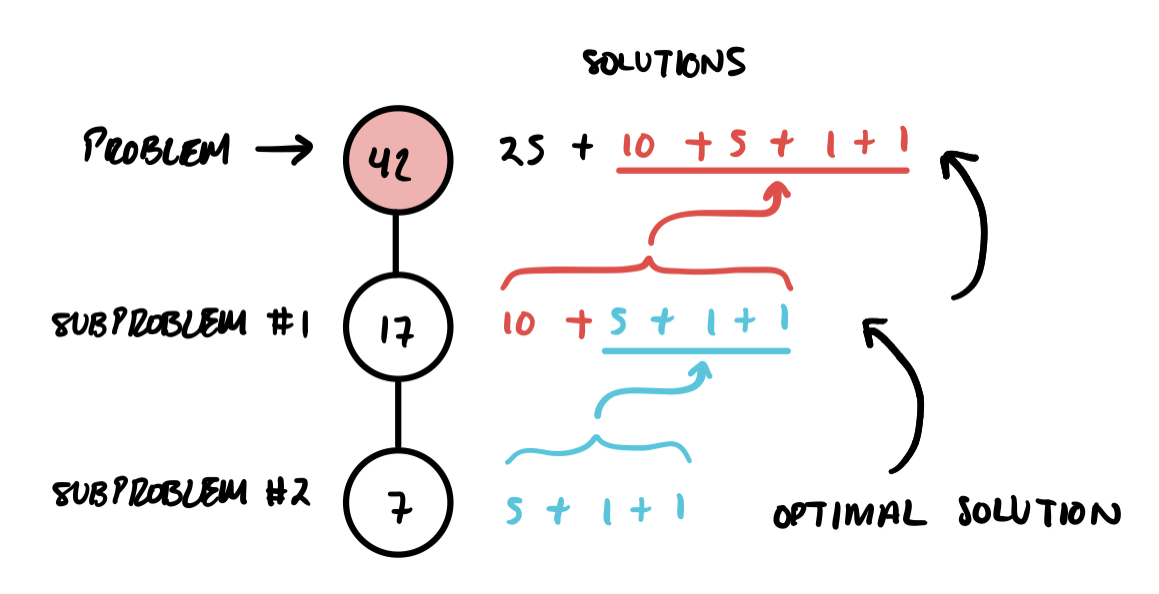
\includegraphics[scale=0.2]{imgs/coin_change_1.jpeg}
    \caption{Optimal solutions to the sub-problems are contained within the global optimal solution}
\end{figure}

\end{frame}


\begin{frame}[fragile]
\frametitle{Greedy - Example \#1: Coin Change}

\begin{enumerate}
	\setcounter{enumi}{1}
    \item \textbf{It has the greedy property}    
    	\begin{itemize}
		    \item For this set of coin denominations (it can be proven) that substracting the largest coin denomination from every amount $V$ that is not greater that the remaining amount, we will always obtain the minimum number of coins (optimal solution)
		\end{itemize}
\end{enumerate}

\begin{figure}
    \centering
    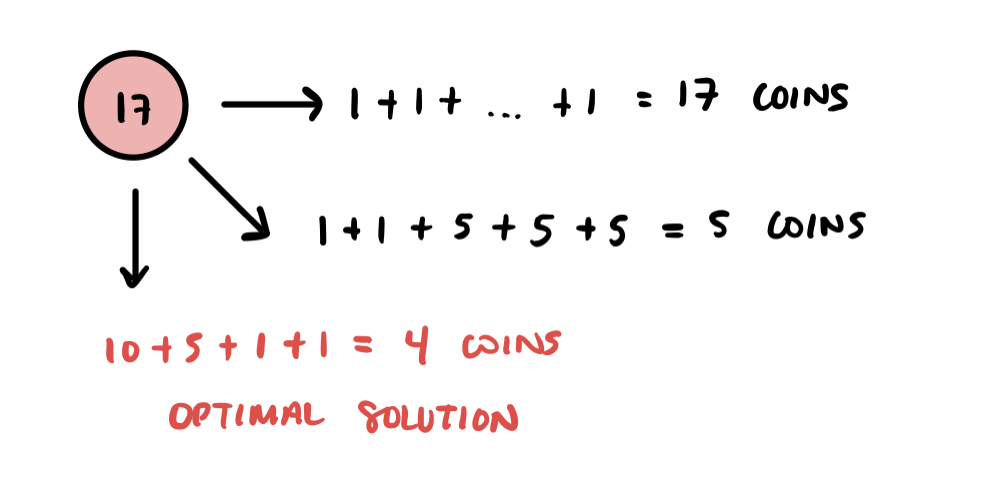
\includegraphics[scale=0.2]{imgs/coin_change_2.jpeg}
    \caption{Substracting the largest coin denomination that is not greater that $V$ will always result in the optimal solution for this set of coins: $\{25,10,5,1\}$}
\end{figure}

\end{frame}

\begin{frame}[fragile]
\frametitle{Greedy - Example \#1: Coin Change}

\begin{itemize}
    \item If we change the set of coins, then the same algorithm might not always result in the optimal solution
    \item For example, take the following set of coins: \verb|{4,3,1}| and $V=6$ cents
    \item Using the previous algorithm, we will obtain that the answer is $4+1+1$, \textbf{3 coins}
    \item Instead of the obvious optimal solution $3+3$, \textbf{2 coins}
\end{itemize}

\vspace{0.3cm}

\color{blue}* The general solution to this problem will be found in \textbf{Dynamic Programming} section\color{black}

\end{frame}

\begin{frame}[fragile]
\frametitle{Greedy - Example \#2: UVa 410 - Station Balance (Load Balancing)}

\color{red}\textbf{Problem description}\color{black} \\

Given $C$ chambers ($1\leq C \leq 5$) which can store $S$ specimens ($1 \leq S \leq 2C$) and a list of $M$ masses (one mass value $i$ per specimen $S_i$), determine which chamber should store each specimen in order to minimize \textbf{imbalance}.

\vspace{0.3cm}

Average total mass in each chamber: $$A = \frac{\sum_{i=1}^{S}M_i}{C}$$

Imbalance: $$I = \sum_{j=1}^{C} |X_j - A|$$ is the sum of differences between the total mass in each chamber $X_j$ with respect to the average total mass $A$

\end{frame}

\begin{frame}[fragile]
\frametitle{Greedy - Example \#2: UVa 410 - Station Balance}

Consider the following values:

\begin{itemize}
    \item $C=3$
    \item $S=4$
    \item $M=\{5,1,2,7\}$
    \item $A=\frac{5+1+2+7}{3} = 5$
\end{itemize}

\begin{figure}
    \centering
    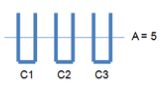
\includegraphics[scale=0.5]{imgs/uva_410_1.png}
\end{figure}

\end{frame}

\begin{frame}[fragile]
\frametitle{Greedy - Example \#2: UVa 410 - Station Balance}

Some possible accomodations: 

\begin{columns}
\column{0.3\textwidth}
	\begin{figure}
    	\centering
	    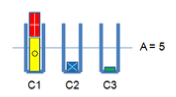
\includegraphics[scale=0.5]{imgs/uva_410_2.png}
    	\caption{$I = 14$}
	\end{figure}

\column{0.3\textwidth}
	\begin{figure}
    	\centering
	    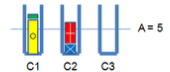
\includegraphics[scale=0.55]{imgs/uva_410_3.png}
    	\caption{$I = 10$}
	\end{figure}

\column{0.3\textwidth}
	\begin{figure}
    	\centering
	    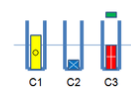
\includegraphics[scale=0.5]{imgs/uva_410_4.png}
    	\caption{$I = 6$}
	\end{figure}

\end{columns}

\begin{itemize}
	\item $M_\text{yellow} = 7$
	\item $M_\text{red} = 5$
	\item $M_\text{blue} = 2$
	\item $M_\text{green} = 1$			
\end{itemize}

\end{frame}

\begin{frame}[fragile]
\frametitle{Greedy - Example \#2: UVa 410 - Station Balance}

\begin{itemize}
    \item Observation 1: If there exists an empty chamber, it's usually beneficial since its worse to have an empty chamber ($I = A$) and its easy to move one specimen with mass $X_j$ to the empty chamber and will have a less imbalance ($I = |A - X_j|$)
    \item \textbf{Observation 2}: If $S>C$, then $S-C$ specimens must be paired with a chamber already containing other specimens\footnote{Pigeonhole principle}
\end{itemize}
\end{frame}

\begin{frame}[fragile]
\frametitle{Greedy - Example \#2: UVa 410 - Station Balance}

Therefore, the solution to the problem can be simplified by sorting:
\begin{enumerate}
    \item If $S<2C$, add $2C - S$ dummy specimens with mass 0
    \item Sort the list $M$
    \item Pair the specimens with masses $M_1$ and $M_{2C}$ into $C_1$
    \item Pair the specimens with masses $M_2$ and $M_{2C-1}$ into $C_2$
    \item $\vdots$
\end{enumerate}

This algorithm is called: \textbf{load balancing}

\end{frame}

\begin{frame}[fragile]
\frametitle{Greedy - Example \#2: UVa 410 - Station Balance}

Returning to the original values: 
\begin{itemize}
    \item $C=3$
    \item $S=4$
    \item $M=\{5,1,2,7\}$
    \item $A=5$
\end{itemize}

\vspace{0.3cm}

\begin{columns}
\column{0.6\textwidth}
	\textbf{Load balancing} algorithm:

	\begin{enumerate}
    	\item $M=\{5,1,2,7,\color{red}0,0\color{black}\}$
	    \item $M=\{0,0,1,2,5,7\}$
    	\item $0$ and $7$ goes in chamber $C_1$
	    \item $0$ and $5$ goes in chamber $C_2$
    	\item $1$ and $2$ goes in chamber $C_3$
	\end{enumerate}
	
\column{0.4\textwidth}
	\begin{figure}
	    \centering
    	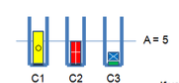
\includegraphics[scale=0.5]{imgs/uva_410_5.png}
	    \caption{Imbalance $I=4$ is optimal}
	\end{figure}

\end{columns}

\end{frame}

\begin{frame}[fragile]
\frametitle{UVa 10382 - Watering Grass (Interval Covering)}

\color{red}\textbf{Problem Description}\color{black} \\
$n$ sprinklers ($n\leq 10000$) are installed in a horizontal strip of grass $L$ meters long and $W$ meters wide. Each sprinkler is centered vertically in the strip. For each sprinkler, we are given its position as the distance from the left end of the center line and its radius of operation. What is the minimum number of sprinklers that should be turned on in order to water the entire strip of grass?

\begin{figure}
    \centering
    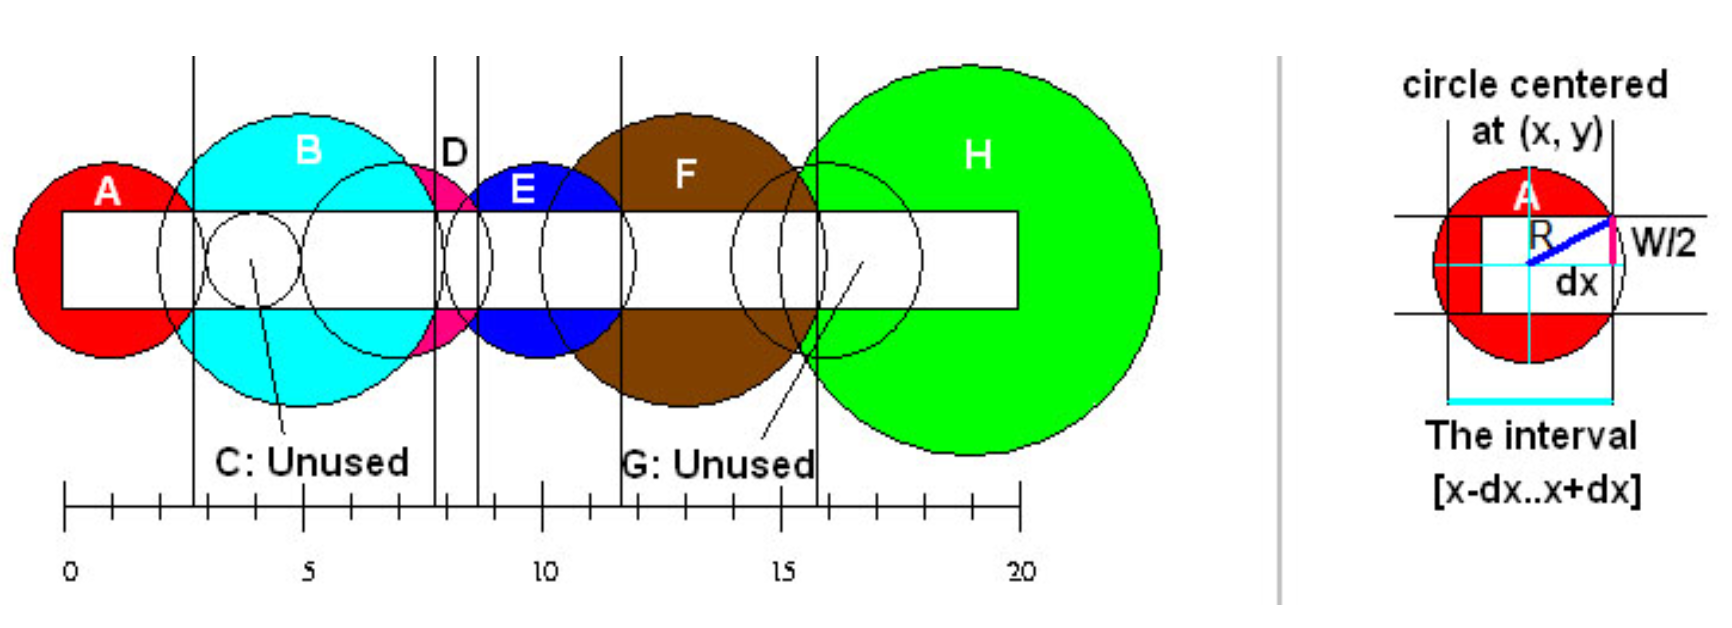
\includegraphics[scale=0.25]{imgs/uva_10382_1.png}
    \caption{UVa 10382 - Watering Grass}
\end{figure}

\end{frame}

\begin{frame}[fragile]
\frametitle{UVa 10382 - Watering Grass}

\begin{columns}
\column{0.7\textwidth}
	\begin{itemize}
	    \item This problem cannot be solved using brute force since $n \leq 10000$ and to solve it we would need to analyze $2^{10000}$ subsets
    	\item This problem is a modification of the \textit{interval covering problem}
	    \item It's possible to transform the circles into the interval covering problem by computing $dx = \sqrt{R^2 - (W/2)^2}$
	\end{itemize}
	
\column{0.3\textwidth}
	\begin{figure}
	    \centering
	    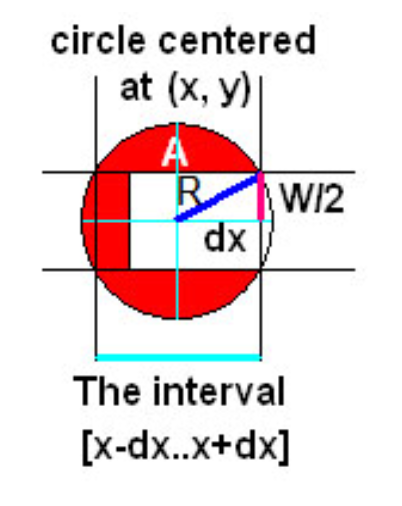
\includegraphics[scale=0.4]{imgs/uva_10382_2.png}
	\end{figure}

\end{columns}
\end{frame}

\begin{frame}[fragile]
\frametitle{UVa 10382 - Watering Grass}

\color{red}\textbf{Solution}\color{black}
\begin{enumerate}
    \item Sort the intervals by increasing left endpoint and decreasing right endpoint if ties arise
    \item Process the intervals one at a time, taking the interval with the largest right endpoint
\end{enumerate} 

\vspace{0.3cm}

*This will produce uninterrupted coverage from the leftmost side to the rightmost side of the horizontal strip of grass, therefore, the minimum number of sprinklers

\end{frame}

\begin{frame}[fragile]
\frametitle{UVa 11292 - Dragon of Lootwater (Sort the Input First)}

\color{red}\textbf{Problem description}\color{black} \\
There are $n$ dragon heads with a specified \textit{diameter} $D$ and $m$ knights with a specified \textit{height} $H$ ($1\leq n,m \leq 20000$). A knight can only chop \textbf{one} dragon head iff $H \geq D$. Given a list of heights and a list of diameters:
\begin{itemize}
    \item Is it possible to chop off all the dragon heads?
    \item If so, what is the minimum total height of the knights used to chop off the dragons' heads?
\end{itemize}

\end{frame}

\begin{frame}[fragile]
\frametitle{UVa 11292 - Dragon of Lootwater}

\color{red}\textbf{Solution}\color{black}\\
\begin{itemize}
    \item This could be thought as a bipartite matching problem
    \item However, this problem can also be solved by sorting the input
    	\begin{itemize}
		    \item Each dragon head should be chopped by a knight with the shortest height that is at least as tall as the diameter of the dragon's head
		    \item Since the input is given in arbitrary order, we could sort both the list of dragon head diameters and knight heights in $O(n\log n + m\log m)$
		    \item Then, we could use the following $O(\text{min}(n,m))$ scan to determine the correct answer
		\end{itemize}
\end{itemize}

\vspace{0.3cm}

\color{red}\verb|C++ code: /Greedy/11292.cpp|\color{black}
\end{frame}

\begin{frame}[fragile]
\frametitle{Greedy in Programming Contests}

\begin{itemize}
    \item For the classical greedy problems (Coin Change, Load Balancing and Interval Covering), it's helpful to memorize their solutionos
    \item When dealing with a greedy problem, it's usually helpful to sort data to highlight hidden greedy strategies
    \item There are two other classical examples of Greedy algorithms:
    	\begin{enumerate}
		    \item Kruskal's (and Prim's) algorithm for the Minimum Spanning Tree (MST)
		    \item Dijkstra's algorithm for the Single-Source Shortest Paths (SSSP)
		\end{enumerate}
	\item A Greedy algorithm won't - normally - encounter TLE verdict, but is more prone to encountering WA verdict
	\item Rule of thumb:
		\begin{itemize}
		    \item If the input size is small enough, use either a Complete Search or Dynamic Programming (DP) approach
		    \item Otherwise, use the Greedy approach
		\end{itemize}
\end{itemize}

\end{frame}

%-------------------------------------------------------------------------------------------
%-------------------------------------------------------------------------------------------
%-------------------------------------------------------------------------------------------
\subsection{UVa - 3.4}
\begin{frame}[fragile]
\frametitle{UVa - Online Judge}
	\begin{itemize}
	    \item Greedy problems: \url{https://onlinejudge.org/index.php?option=com_onlinejudge&Itemid=8&category=656}
	    \item If site is not working, please refer to \cite{Halim}: page 93 and 94 for Greedy problems
	\end{itemize}
\end{frame}


%-------------------------------------------------------------------------------------------
%-------------------------------------------------------------------------------------------
%-------------------------------------------------------------------------------------------
\section{8.2 More Advanced Search Techniques}

\begin{frame}[fragile]
\frametitle{8.2 More Advanced Search Techniques}

We have already seen iterative and recursive backtracking Complete Search techniques. However, some problems require other search techniques to avoid the TLE\footnote{Time Limit Exceeded} verdict. 

\end{frame}

\begin{frame}[fragile]
\frametitle{8.2.1 Backtracking with Bitmask}

Recall that a bitmask can be used to model a small set of Boolean. Bitmask operations are very lightweight and we could use them to speed up a Complete Search solution.

\end{frame}

\begin{frame}[fragile]
\frametitle{UVa 11195 - Another n-Queen Problem}

\begin{itemize}
    \item UVa 11195 would still get a TLE even when using the three bitsets \verb|rw, ld, rd| from the previous formulation (section 3.2 - Recursive Complete Search)
    \item First, let's use bitmasks instead of bitsets for representing the three sets of Booleans
    \item These bitmasks represent which rows are attacked (or, not available to place another queen) in the next column, left and right diagonal from previously placed queens
\end{itemize}

\end{frame}

\begin{frame}[fragile]
\frametitle{UVa 11195 - Another n-Queen Problem}

\begin{lstlisting}[language=C]
int ans = 0, OK = (1 << 5) - 1;
void backtrack(int rw, int ld, int rd) {
	// if all bits in rw are on
	if (rw == OK) { ans++; return; } 
	// the ones in pos mean availability
	int pos = OK & (~(rw | ld | rd));
	while (pos) {
		// p will be the Least Significant One
		int p = pos & -pos;
		// turn off the LSO
		pos -= p;
		backtrack(rw | p, (ld | p) << 1, (rd | p) >> 1);
	}
}
int main() {
	backtrack(0,0,0);
	printf("\%d\n", ans);
}

\end{lstlisting}

\end{frame}

\begin{frame}[fragile]
\frametitle{UVa 11195 - Another n-Queen Problem}

Let's see how this works:

\begin{figure}
    \centering
    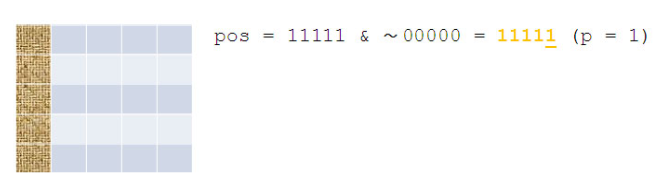
\includegraphics[scale=0.6]{imgs/nqueen_0.png}
    \caption{Initial state}
\end{figure}

\begin{figure}
    \centering
    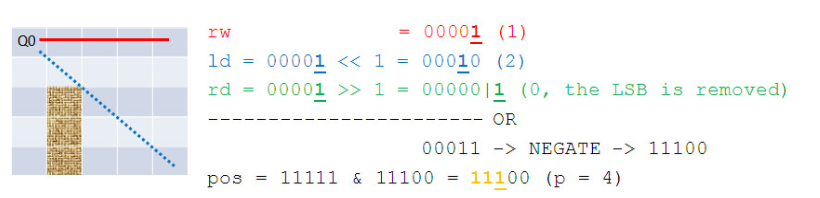
\includegraphics[scale=0.6]{imgs/nqueen_1.png}
    \caption{After positioning the first queen, \textbf{pos} only reflects the three available spots for the second queen in the second column}
\end{figure}

\end{frame}

\begin{frame}[fragile]
\frametitle{UVa 11195 - Another n-Queen Problem}

\begin{figure}
    \centering
    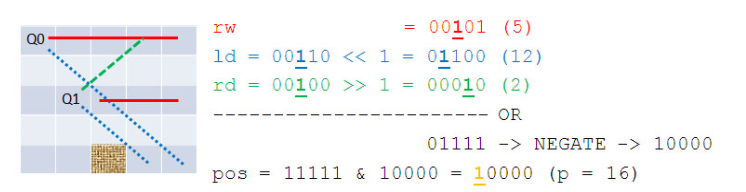
\includegraphics[scale=0.6]{imgs/nqueen_2.png}
    \caption{After positioning the second queen, \textbf{ld} reflects this change by turning on bits 2 and 3 (which corresponds to row 2 and 3 respectively). The same thing happens with \textbf{rd} but with row 1}
\end{figure}

\begin{figure}
    \centering
    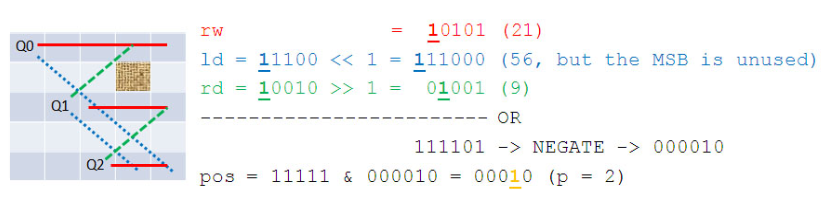
\includegraphics[scale=0.6]{imgs/nqueen_3.png}
\end{figure}

\end{frame}

\begin{frame}[fragile]
\frametitle{UVa 11195 - Another n-Queen Problem}

\begin{figure}
    \centering
    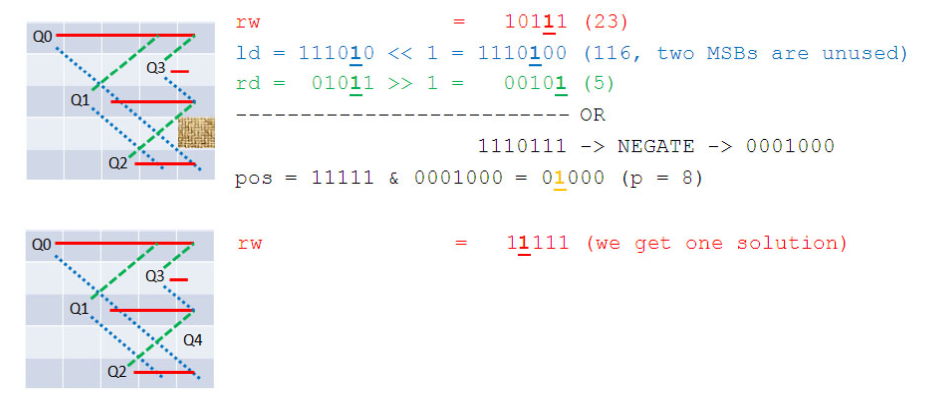
\includegraphics[scale=0.6]{imgs/nqueen_4.png}
    \caption{Final solution when \textbf{rw} has all five bits turned on}
\end{figure}

\end{frame}

\begin{frame}[fragile]
\frametitle{8.2.2 Backtracking with Heavy Prunning}

\color{red}Problem description\color{black} \\

Given an $M \times N$ board with $3$ check-in points $\{A, B, C\}$, find a Hamiltonian path\footnote{Path in an undirected graph that visits each vertex exactly once} of length $(M \times N)$ from coordinate $(0, 0)$ to coordinate $(0, 1)$. This Hamiltonian path must hit the three check points: $A$, $B$, and $C$ at one-quarter, one-half, and three-quarters of the way through its path, respectively. Constraints: $2 \leq M, N \leq 8$.

\end{frame}

\begin{frame}[fragile]
\frametitle{Backtracking with Heavy Prunning}

For example, $3 \times 6$ board with $A=(2,1)$, $B=(2,4)$ and $C=(0,4)$, we have two options: 

\begin{figure}
    \centering
    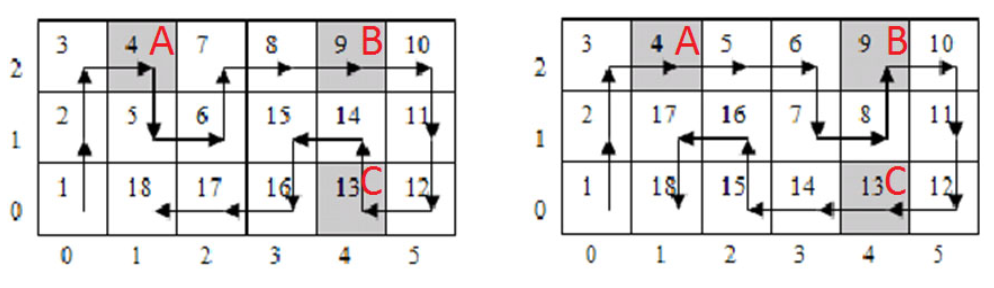
\includegraphics[scale=0.5]{imgs/robots_on_ice.png}
\end{figure}

\end{frame}

\begin{frame}[fragile]
\frametitle{Backtracking with Heavy Prunning}

\textbf{Naive solution}: try with all paths and exit when found a Hamiltonian path. To implement this solution, we would need - in the worst case - to analyze $4^{64} = 3.4\times10^{38}$ paths, which is simply unfeasible.

\end{frame}

\begin{frame}[fragile]
\frametitle{Backtracking with Heavy Prunning}

\textbf{Heavy Prunning}: prune the search space if the search:
\begin{enumerate}
    \item Wanders outside the $M\times N$ grid
    \item Does not hit the appropriate target check point at one-quarter, one-half and three-quarters distace
    \item Hits target check point earlier than the target distance
    \item Will not be able to hit certain coordinates as the current partial path self-blocks the access to those coordinates. This can be checked with a simple DFS/BFS starting from coordinates $(0,1)$ and determine if there are coordinates in the grid that are not reachable from $(0,1)$ and not yet visited by the current partial path, we can prune the current partial path
\end{enumerate}

\end{frame}


%-------------------------------------------------------------------------------------------
%-------------------------------------------------------------------------------------------
%-------------------------------------------------------------------------------------------
\subsection{UVa - 8.2}
\begin{frame}[fragile]
\frametitle{UVa - Online Judge}
	\begin{itemize}
	    \item More Advanced Search problems: \url{https://onlinejudge.org/index.php?option=com_onlinejudge&Itemid=8&category=765}
	    \item If site is down, please refer to \cite{Halim}: page 310 and 311 for this section's problems
	\end{itemize}
\end{frame}


%-------------------------------------------------------------------------------------------
%-------------------------------------------------------------------------------------------
%-------------------------------------------------------------------------------------------
\section*{References}
\begin{frame}{References}
    \begin{thebibliography}{}
        \bibitem[Halim]{Halim} Halim S., Halim F., \textit{Competitive Programming 3}, Handbook for ACM ICPC and IOI Contestants. 2013
        \bibitem[Skiean]{Skiena} Skiena S. \textit{The Algorithm Design Manual}. Springer. 2020
        \bibitem[Martinez]{Martinez} Martínez L. \textit{Apuntes de Matemáticas Discretas y Algoritmos}. Instituto de Investigaciones en Matemáticas Aplicadas y Sistemas. 2020
    \end{thebibliography}
\end{frame}

\end{document}
